%
% quadratur.tex
%
% (c) 2021 Prof Dr Andreas Müller, OST Ostschweizer Fachhochschule
%
\begin{frame}[t]
\frametitle{Quadratur des Kreises}
\vspace{-20pt}
\begin{columns}[t,onlytextwidth]
\begin{column}{0.44\textwidth}
\begin{center}
\uncover<2->{%
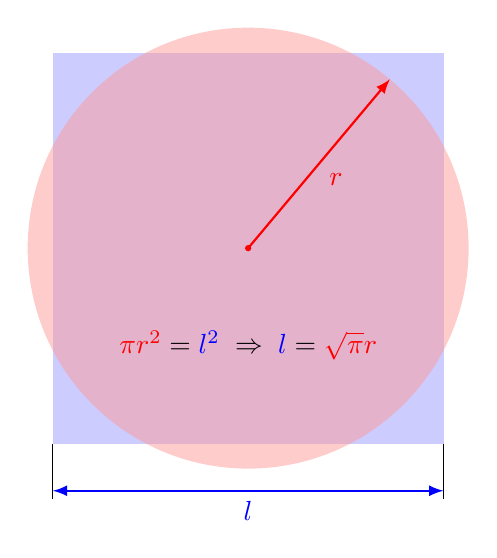
\begin{tikzpicture}[>=latex,thick]

\def\r{2.8}
\pgfmathparse{sqrt(3.14159)*\r/2}
\xdef\s{\pgfmathresult}

\fill[color=blue!20] (-\s,-\s) rectangle (\s,\s);
\fill[color=red!40,opacity=0.5] (0,0) circle[radius=\r];

\uncover<3->{
	\draw[->,color=red] (0,0) -- (50:\r);
	\fill[color=red] (0,0) circle[radius=0.04];
	\node[color=red] at (50:{0.5*\r}) [below right] {$r$};
}

\uncover<4->{
	\draw[line width=0.3pt] (-\s,-\s) -- (-\s,{-\s-0.7});
	\draw[line width=0.3pt] (\s,-\s) -- (\s,{-\s-0.7});
	\draw[<->,color=blue] (-\s,{-\s-0.6}) -- (\s,{-\s-0.6});
	\node[color=blue] at (0,{-\s-0.6}) [below] {$l$};
}

\uncover<5->{
	\node at (0,{-\s/2}) {${\color{red}\pi r^2}={\color{blue}l^2}
		\;\Rightarrow\;
		{\color{blue}l}={\color{red}\sqrt{\pi}r}$};
}

\end{tikzpicture}}
\end{center}
\end{column}
\begin{column}{0.52\textwidth}
\begin{block}{Aufgabe}
Konstruiere ein zu einem Kreis flächengleiches Quadrat
\end{block}
\uncover<6->{%
\begin{block}{Modifizierte Aufgabe}
Konstruiere eine Strecke, deren Länge Lösung der Gleichung
$x^2-\pi=0$ ist.
\end{block}}
\uncover<7->{%
\begin{proof}[Unmöglichkeitsbeweis mit Widerspruch]
\begin{itemize}
\item<8-> Lösung in einem Erweiterungskörper
\item<9-> Lösung ist Nullstelle eines Polynoms 
\item<10-> Lösung ist algebraisch
\item<11-> $\pi$ ist {\bf nicht} algebraisch
\uncover<12->{(Lindemann 1882\only<13>{, Weierstrass 1885})}
\qedhere
\end{itemize}
\end{proof}}
\end{column}
\end{columns}
\end{frame}
